\documentclass[ignorenonframetext,]{beamer}
\setbeamertemplate{caption}[numbered]
\setbeamertemplate{caption label separator}{: }
\setbeamercolor{caption name}{fg=normal text.fg}
\beamertemplatenavigationsymbolsempty
\usepackage{lmodern}
\usepackage{amssymb,amsmath}
\usepackage{ifxetex,ifluatex}
\usepackage{fixltx2e} % provides \textsubscript
\ifnum 0\ifxetex 1\fi\ifluatex 1\fi=0 % if pdftex
  \usepackage[T1]{fontenc}
  \usepackage[utf8]{inputenc}
\else % if luatex or xelatex
  \ifxetex
    \usepackage{mathspec}
  \else
    \usepackage{fontspec}
  \fi
  \defaultfontfeatures{Ligatures=TeX,Scale=MatchLowercase}
\fi
\usetheme[]{Luebeck}
\usecolortheme{seagull}
\usefonttheme{structurebold}
% use upquote if available, for straight quotes in verbatim environments
\IfFileExists{upquote.sty}{\usepackage{upquote}}{}
% use microtype if available
\IfFileExists{microtype.sty}{%
\usepackage{microtype}
\UseMicrotypeSet[protrusion]{basicmath} % disable protrusion for tt fonts
}{}
\newif\ifbibliography
\hypersetup{
            pdftitle={Causes and consequences of adaptation to environmental change},
            pdfauthor={Pratik Gupte},
            pdfborder={0 0 0},
            breaklinks=true}
\urlstyle{same}  % don't use monospace font for urls
\usepackage{graphicx,grffile}
\makeatletter
\def\maxwidth{\ifdim\Gin@nat@width>\linewidth\linewidth\else\Gin@nat@width\fi}
\def\maxheight{\ifdim\Gin@nat@height>\textheight0.8\textheight\else\Gin@nat@height\fi}
\makeatother
% Scale images if necessary, so that they will not overflow the page
% margins by default, and it is still possible to overwrite the defaults
% using explicit options in \includegraphics[width, height, ...]{}
\setkeys{Gin}{width=\maxwidth,height=\maxheight,keepaspectratio}

% Prevent slide breaks in the middle of a paragraph:
\widowpenalties 1 10000
\raggedbottom

\AtBeginPart{
  \let\insertpartnumber\relax
  \let\partname\relax
  \frame{\partpage}
}
\AtBeginSection{
  \ifbibliography
  \else
    \let\insertsectionnumber\relax
    \let\sectionname\relax
    \frame{\sectionpage}
  \fi
}
\AtBeginSubsection{
  \let\insertsubsectionnumber\relax
  \let\subsectionname\relax
  \frame{\subsectionpage}
}

\setlength{\parindent}{0pt}
\setlength{\parskip}{6pt plus 2pt minus 1pt}
\setlength{\emergencystretch}{3em}  % prevent overfull lines
\providecommand{\tightlist}{%
  \setlength{\itemsep}{0pt}\setlength{\parskip}{0pt}}
\setcounter{secnumdepth}{0}

\title{Causes and consequences of adaptation to environmental change}
\author{Pratik Gupte}
\date{11 July 2018}

\begin{document}
\frame{\titlepage}

\begin{frame}{Environmental change \& reaction norms}

The \textbf{temporal scale} and \textbf{predictability} of environmental
change can vary.\footnote<.->{Botero et al. (2015).}

\includegraphics[width=0.6\linewidth]{botero_fig1}

\end{frame}

\begin{frame}{Environment change \& behaviour}

How does this affect:

\begin{itemize}
\tightlist
\item
  Distribution of behavioural traits?
\item
  Adaptive strategies?
\end{itemize}

\end{frame}

\begin{frame}{Exploratory behaviour in red knots}

\begin{itemize}
\tightlist
\item
  Wintering knots: consistent differences in exploratory
  behaviour\footnote<.->{Bijleveld et al. (2014).}
\end{itemize}

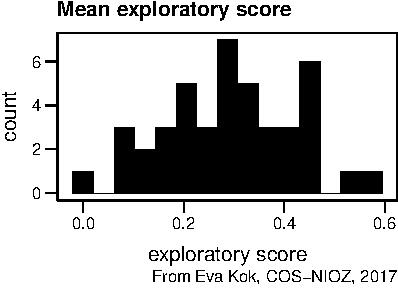
\includegraphics{pres_pg_11072018_files/figure-beamer/plot-1.pdf}

\end{frame}

\begin{frame}{Refs}

\hypertarget{refs}{}
\hypertarget{ref-bijleveld_personality_2014}{}
Bijleveld AI, Massourakis G, Marel A van der et al. (2014) Personality
drives physiological adjustments and is not related to survival.
Proceedings of the Royal Society of London B: Biological Sciences
281:20133135. doi:
\href{https://doi.org/10.1098/rspb.2013.3135}{10.1098/rspb.2013.3135}

\hypertarget{ref-botero_evolutionary_2015}{}
Botero CA, Weissing FJ, Wright J, Rubenstein DR (2015) Evolutionary
tipping points in the capacity to adapt to environmental change.
Proceedings of the National Academy of Sciences 112:184--189. doi:
\href{https://doi.org/10.1073/pnas.1408589111}{10.1073/pnas.1408589111}

\end{frame}

\end{document}
